\chapter{Object-Oriented Structural Analysis Program}

\section{Introduction}
This project develops a 2D structural analysis program using the Direct Stiffness Method (DSM) with an object-oriented design. The implementation supports frame and truss elements in a unified 3-DOF-per-node formulation (\(u_x, u_y, r_z\)) and computes nodal displacements, support reactions, and member-end forces under static loading.

The main objective is to provide a reusable and extensible solver architecture for CE4011 assignments, while preserving numerical efficiency by reusing the matrix library from Q1.

\subsection*{File Architecture}
To keep the GitHub repository focused and easy to navigate, the project is organized around a small set of source, analysis, and report files:
\begin{itemize}
  \item \textbf{Report root}: \texttt{main.tex} assembles the full report, while \texttt{Chapter1\_...tex} through \texttt{Chapter5\_...tex} contain the chapter content.
  \item \textbf{Structural solver}: \texttt{q2\_frame\_analysis/} contains the solver implementation, models, tests, regression cases, and generated results.
  \item \textbf{Shared numerics}: \texttt{q1\_matrix\_library/} stores the reusable sparse matrix and solver utilities imported from the earlier assignment.
  \item \textbf{Assets and outputs}: figures, screenshots, and exported logs are kept in dedicated folders such as \texttt{images/}, \texttt{ftool/}, and \texttt{results/} so the codebase stays compact.
\end{itemize}
This layout reduces clutter, keeps the solver code separated from report assets, and makes the GitHub repository easier to review and maintain.

\section{Analysis and Design Decisions}
\subsection*{Why Object-Oriented Programming (OOP)}
OOP was selected to separate responsibilities and improve maintainability:
\begin{itemize}
    \item \textbf{Modeling clarity:} classes such as \texttt{Node}, \texttt{Element}, and \texttt{Structure} map directly to engineering entities.
    \item \textbf{Extensibility:} new element types or load models can be added by subclassing without redesigning the full solver.
    \item \textbf{Encapsulation:} geometry, stiffness, load conversion, and post-processing logic stay close to the associated class.
\end{itemize}

\subsection*{Why Direct Stiffness Method (DSM)}
DSM is the standard finite-element formulation for linear structural analysis:
\begin{itemize}
    \item naturally supports mixed element assemblies,
    \item gives a systematic global matrix equation \(\mathbf{K}\mathbf{d}=\mathbf{F}\),
    \item aligns with sparse matrix assembly and iterative solution techniques.
\end{itemize}

\subsection*{Why Reuse the Q1 Matrix Library}
The Q1 implementation (symmetric sparse matrix, vector, and conjugate gradient solver) from Assignment 2 was reused because:
\begin{itemize}
    \item stiffness matrices are symmetric by formulation,
    \item sparse storage reduces memory usage,
    \item conjugate gradient is appropriate for large symmetric systems,
    \item it preserves continuity between Q1 and Q2 deliverables.
\end{itemize}

\subsection*{Why a Frame/Truss Hierarchy}
A base \texttt{Element} abstraction defines shared behavior (geometry transforms, global mapping), while subclasses implement element-specific mechanics:
\begin{itemize}
    \item \texttt{FrameElement}: axial + flexural stiffness, optional end releases, member-load fixed-end effects.
    \item \texttt{TrussElement}: axial-only stiffness embedded in the same 6-DOF element format.
\end{itemize}
This avoids duplicate code and preserves a consistent assembly interface.

\section{UML Class Diagram}
The architecture of the structural analysis program is organised into three
logical layers: a \textbf{numerical library layer} (\texttt{SymmetricSparseMatrix},
\texttt{Vector}, \texttt{ConjugateGradientSolver}), a \textbf{model layer}
(\texttt{Node}, \texttt{Material}, \texttt{Section}, \texttt{Element},
\texttt{FrameElement}, \texttt{TrussElement}), and an \textbf{analysis
coordination layer} (\texttt{Structure}).
The full class diagram is presented in Figure~\ref{fig:uml}, and each
relationship is described in detail below.

\begin{figure}[h!]
\centering
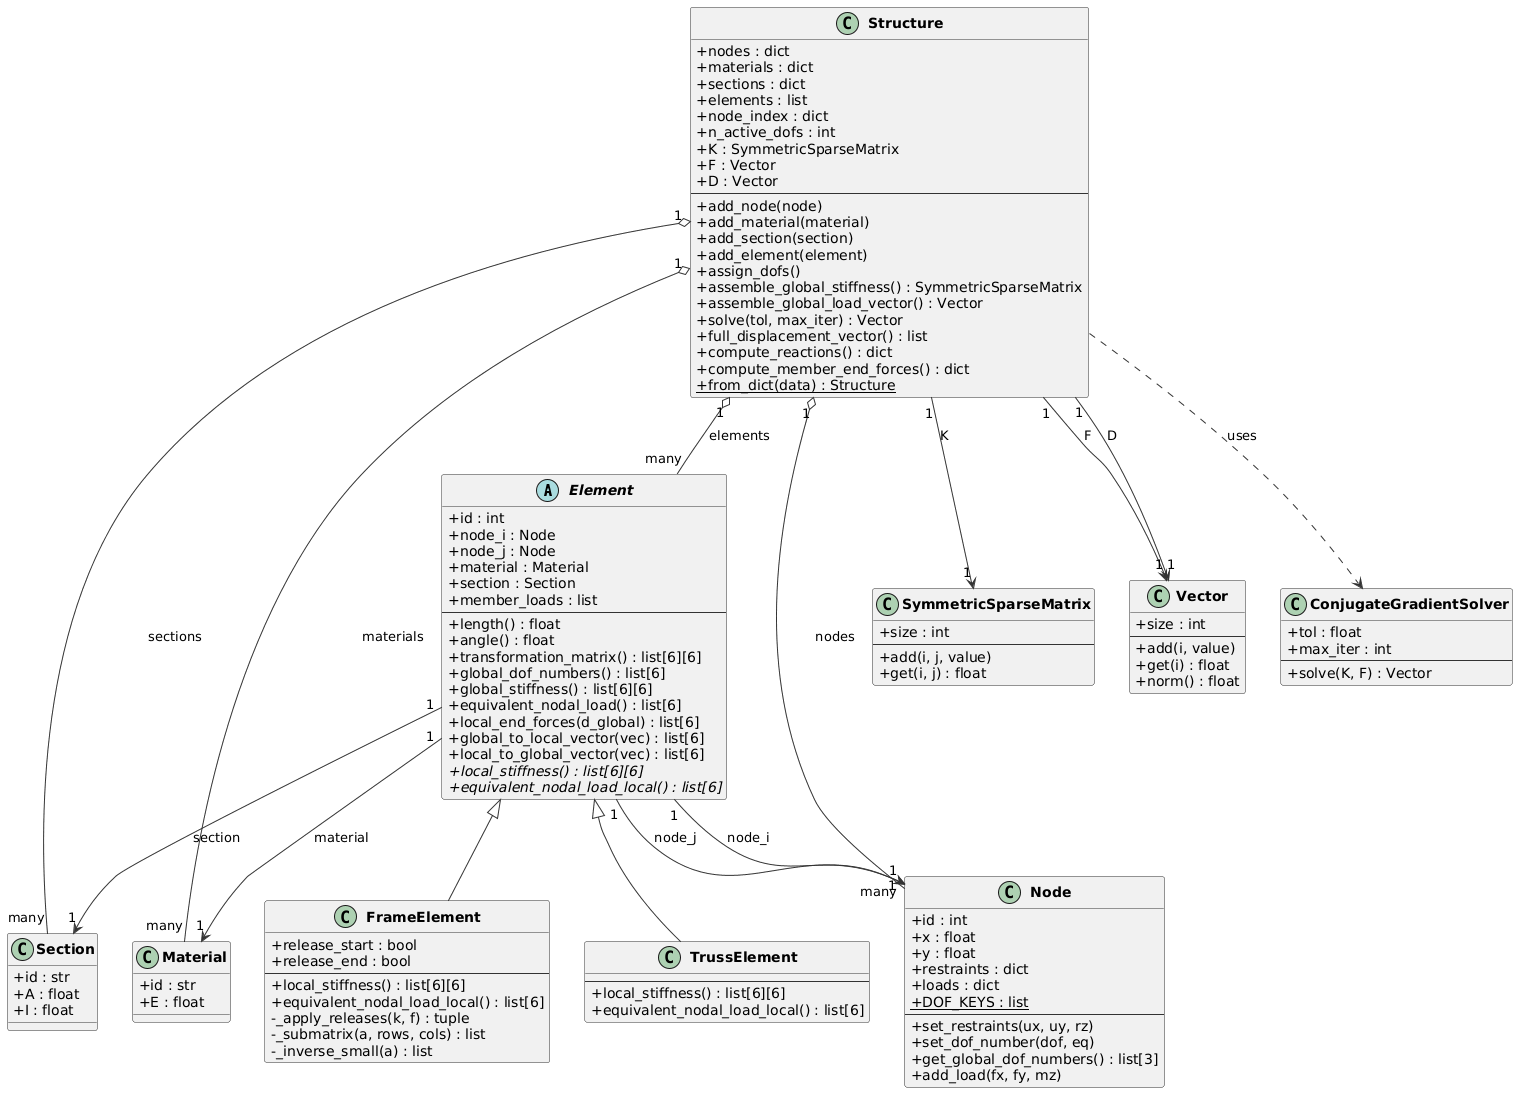
\includegraphics[width=\textwidth]{uml.png}
\caption{UML class diagram of the structural analysis program}
\label{fig:uml}
\end{figure}

% ------------------------------------------------------------------
\subsection*{Inheritance and Abstraction}
% ------------------------------------------------------------------

\texttt{Element} is defined as an \textbf{abstract base class}.
It declares two abstract methods that every concrete element type must
implement: \texttt{local\_stiffness()} and
\texttt{equivalent\_nodal\_load\_local()}.
All remaining behaviour --- coordinate transformation, global stiffness
assembly, equivalent load transformation, and member-end force recovery ---
is implemented once in \texttt{Element} and inherited by every subclass.
This is a direct application of the \textbf{Template Method} pattern: the
base class defines the algorithm skeleton while subclasses supply the
element-specific steps.

\texttt{FrameElement} and \texttt{TrussElement} each participate in a
\textbf{generalisation / specialisation} (is-a) relationship with
\texttt{Element}:

\begin{itemize}
  \item \texttt{FrameElement} \textbf{is-a} \texttt{Element}.
  It specialises the base class by implementing full axial and flexural
  stiffness, optional moment releases at either end via static
  condensation, and fixed-end force vectors for transverse point loads
  and uniformly distributed loads.

  \item \texttt{TrussElement} \textbf{is-a} \texttt{Element}.
  It specialises the base class by restricting stiffness to the axial
  direction only. Rotational and transverse degrees of freedom receive
  zero stiffness contributions, and only axial member loads are
  accepted.
\end{itemize}

In UML notation both relationships are represented by a solid line with a
hollow triangular arrowhead pointing from the subclass to the abstract
parent, indicating that the subclass inherits the interface and all
non-abstract behaviour of \texttt{Element}.

% ------------------------------------------------------------------
\subsection*{Encapsulation}
% ------------------------------------------------------------------

Encapsulation is enforced at two levels throughout the design.

At the \textbf{element level}, the internal condensation helpers of
\texttt{FrameElement} --- \texttt{\_apply\_releases()},
\texttt{\_submatrix()}, \texttt{\_inverse\_small()},
\texttt{\_mat\_mul()}, \texttt{\_mat\_sub()}, \texttt{\_mat\_vec()}, and
\texttt{\_vec\_sub()} --- are prefixed with an underscore to signal that
they are private implementation details.
External callers interact only with the public interface defined on
\texttt{Element}.
This prevents the release-condensation logic from leaking into the
assembly or postprocessing routines.

At the \textbf{structure level}, \texttt{Structure} holds its internal
state (\texttt{K}, \texttt{F}, \texttt{D}, \texttt{node\_index},
\texttt{n\_active\_dofs}) privately and exposes behaviour only through
well-defined methods (\texttt{assemble\_global\_stiffness()},
\texttt{solve()}, \texttt{compute\_reactions()},
\texttt{compute\_member\_end\_forces()}).
No external code is required to manipulate the stiffness matrix or
displacement vector directly.

% ------------------------------------------------------------------
\subsection*{Modularity}
% ------------------------------------------------------------------

The program is partitioned into three independently maintainable modules.

\begin{itemize}
  \item \textbf{matrixlib}: provides \texttt{SymmetricSparseMatrix},
  \texttt{Vector}, and \texttt{ConjugateGradientSolver}.
  This module has no dependency on structural mechanics and can be
  reused for any symmetric linear system.

  \item \textbf{model}: contains all structural classes.
  \texttt{Element} and its subclasses depend on \texttt{Node},
  \texttt{Material}, and \texttt{Section} for geometric and physical
  data, but have no knowledge of \texttt{Structure} or the numerical
  library.

  \item \textbf{analysis coordination}: \texttt{Structure} imports from
  both \texttt{model} and \texttt{matrixlib} but is not imported by
  either.
  This one-way dependency ensures that changes to the numerical solver
  or element formulations do not cascade into each other.
\end{itemize}

% ------------------------------------------------------------------
\subsection*{Class-by-Class Relationship Analysis}
% ------------------------------------------------------------------

\paragraph{Node.}
\texttt{Node} is a \textbf{data-bearing entity} that stores coordinates,
restraint flags, applied nodal loads, and global degree-of-freedom
equation numbers.
It has no dependency on any other class in the system.
\texttt{Node} is referenced by \texttt{Element} (two associations) and
owned in aggregate by \texttt{Structure} (aggregation).
\texttt{Node} exposes \texttt{DOF\_KEYS} as a class-level constant, making
the degree-of-freedom ordering (\texttt{ux}, \texttt{uy}, \texttt{rz})
part of the class contract rather than a convention scattered across
callers.

\paragraph{Material.}
\texttt{Material} is a simple value object holding the elastic modulus
\texttt{E}.
It participates in a \textbf{1:1 association} with each \texttt{Element}
instance: one element references exactly one material.
Multiple elements may reference the same \texttt{Material} object, making
the relationship from \texttt{Material} to \texttt{Element} effectively
\textbf{1:Many} across the model, though \texttt{Material} itself carries
no back-reference.
\texttt{Material} is stored and managed by \texttt{Structure}.

\paragraph{Section.}
\texttt{Section} holds the cross-sectional properties \texttt{A} and
\texttt{I}.
Its relationship structure is identical to that of \texttt{Material}: a
\textbf{1:1 association} to each \texttt{Element} at the instance level,
and a potential \textbf{1:Many} relationship across the full model when
a single section is shared by multiple elements.
\texttt{Structure} owns the section registry.

\paragraph{Element (abstract).}
\texttt{Element} participates in the following relationships:

\begin{itemize}
  \item \textbf{Association to Node (1:1, twice)}.
  Each \texttt{Element} holds exactly one reference to \texttt{node\_i}
  and one to \texttt{node\_j}.
  These references are set at construction time and do not change,
  making them navigable associations rather than aggregations:
  \texttt{Element} uses the node but does not own it.
  The multiplicity from \texttt{Element} to each \texttt{Node} is
  therefore \textbf{Many:1} across the model, since many elements can
  share the same node.

  \item \textbf{Association to Material (Many:1)}.
  Many elements may share one material definition.

  \item \textbf{Association to Section (Many:1)}.
  Many elements may share one section definition.

  \item \textbf{Generalisation to FrameElement and TrussElement}.
  Described above under Inheritance.
\end{itemize}

The \texttt{member\_loads} attribute is a Python list owned by each
\texttt{Element} instance.
It represents a \textbf{whole/part} (composition) relationship between
\texttt{Element} and the load dictionaries: the loads have no existence
independent of the element that carries them.
In UML this is a filled diamond on the \texttt{Element} side.

\paragraph{FrameElement.}
Beyond the inherited relationships, \texttt{FrameElement} introduces two
boolean attributes (\texttt{release\_start}, \texttt{release\_end}) that
control internal behaviour via \texttt{\_apply\_releases()}.
This method performs static condensation of the local stiffness matrix and
the fixed-end force vector simultaneously when one or both moment releases
are active.
The condensation helpers are entirely internal: no other class calls them
directly, preserving the encapsulation boundary.

\paragraph{TrussElement.}
\texttt{TrussElement} adds no new attributes beyond what \texttt{Element}
provides.
Its specialisation is purely behavioural: \texttt{local\_stiffness()}
returns a matrix with nonzero entries only at positions \texttt{(0,0)},
\texttt{(0,3)}, \texttt{(3,0)}, and \texttt{(3,3)}, and
\texttt{equivalent\_nodal\_load\_local()} rejects any non-axial load
direction with an explicit error.

\paragraph{Structure.}
\texttt{Structure} is the central coordinator and participates in the
largest number of relationships:

\begin{itemize}
  \item \textbf{Aggregation of Node (1:Many)}.
  \texttt{Structure} owns a dictionary of \texttt{Node} objects.
  The multiplicity is \textbf{1:Many}: one structure contains many
  nodes.
  This is an aggregation (hollow diamond) rather than a composition
  because, in principle, \texttt{Node} objects could exist and be
  inspected independently of the \texttt{Structure} that manages them.

  \item \textbf{Aggregation of Material (1:Many)}.
  \texttt{Structure} maintains a material registry.
  Multiplicity is \textbf{1:Many}.

  \item \textbf{Aggregation of Section (1:Many)}.
  \texttt{Structure} maintains a section registry.
  Multiplicity is \textbf{1:Many}.

  \item \textbf{Aggregation of Element (1:Many)}.
  \texttt{Structure} owns the element list.
  Multiplicity is \textbf{1:Many}.
  This is the primary whole/part relationship in the model layer:
  elements are created for and managed by a specific structure.

  \item \textbf{Association to SymmetricSparseMatrix (1:1)}.
  After assembly, \texttt{Structure} holds one instance of
  \texttt{SymmetricSparseMatrix} as its global stiffness matrix
  \texttt{K}.
  Before \texttt{assemble\_global\_stiffness()} is called, \texttt{K}
  is \texttt{None}, so the association is conditional on the analysis
  state.

  \item \textbf{Association to Vector (1:1, twice)}.
  \texttt{Structure} holds \texttt{F} (load vector) and \texttt{D}
  (displacement solution), each a \texttt{Vector} instance, after the
  respective assembly and solve steps.

  \item \textbf{Dependency on ConjugateGradientSolver}.
  \texttt{Structure.solve()} instantiates a
  \texttt{ConjugateGradientSolver} locally, uses it to solve the
  system, and discards it.
  This is a \textbf{dependency} (dashed arrow) rather than an
  association, because the solver is not stored as an attribute of
  \texttt{Structure}.
  The relationship is \textbf{transient}: it exists only for the
  duration of the \texttt{solve()} call.

  \item \textbf{Static factory method \texttt{from\_dict()}}.
  This class method acts as a \textbf{factory}: it receives a raw
  dictionary, constructs all \texttt{Node}, \texttt{Material},
  \texttt{Section}, and \texttt{Element} instances, and returns a fully
  initialised \texttt{Structure}.
  This centralises object initialisation and is the only path through
  which JSON input enters the object model.
  In UML it is shown as a static method on \texttt{Structure} with a
  return type of \texttt{Structure}.
\end{itemize}

% ------------------------------------------------------------------
\subsection*{Hierarchy Summary}
% ------------------------------------------------------------------

The class hierarchy has two levels of depth:

\begin{enumerate}
  \item \textbf{Abstract root}: \texttt{Element} defines the element
  interface and shared geometry behaviour.
  \item \textbf{Concrete leaves}: \texttt{FrameElement} and
  \texttt{TrussElement} implement element-specific mechanics.
\end{enumerate}

No further subclassing is anticipated within the current scope.
The hierarchy is intentionally shallow to keep the design navigable and
to avoid the fragile-base-class problems that arise from deep inheritance
chains.

% ------------------------------------------------------------------
\subsection*{Multiplicity Summary Table}
% ------------------------------------------------------------------

\begin{table}[h!]
\centering
\caption{Summary of class relationship multiplicities}
\begin{tabular}{llll}
\hline
\textbf{From} & \textbf{To} & \textbf{Type} & \textbf{Multiplicity} \\
\hline
FrameElement   & Element              & Generalisation     & Many:1  \\
TrussElement   & Element              & Generalisation     & Many:1  \\
Element        & Node (node\_i)       & Association        & Many:1  \\
Element        & Node (node\_j)       & Association        & Many:1  \\
Element        & Material             & Association        & Many:1  \\
Element        & Section              & Association        & Many:1  \\
Element        & member\_loads        & Composition        & 1:Many  \\
Structure      & Node                 & Aggregation        & 1:Many  \\
Structure      & Material             & Aggregation        & 1:Many  \\
Structure      & Section              & Aggregation        & 1:Many  \\
Structure      & Element              & Aggregation        & 1:Many  \\
Structure      & SymmetricSparseMatrix& Association        & 1:1     \\
Structure      & Vector (F)           & Association        & 1:1     \\
Structure      & Vector (D)           & Association        & 1:1     \\
Structure      & ConjugateGradientSolver & Dependency      & transient \\
\hline
\end{tabular}
\label{tab:multiplicities}
\end{table}


\section{Analysis Assumptions}
The current solver is based on the following assumptions:
\begin{itemize}
    \item Linear elastic material behavior.
    \item Small displacement and small rotation kinematics.
    \item Static loading (no inertia or damping effects).
    \item 2D planar structural behavior.
    \item Euler-Bernoulli frame behavior (no shear deformation in frame elements).
    \item Truss elements carry axial force only.
    \item Supports/restraints are modeled as prescribed zero DOFs.
\end{itemize}

\section{Input Format}

The solver accepts input in JSON format. The input defines the structural model through nodes, materials, sections, elements, and loads.

The required fields are summarized below:

\begin{itemize}
    \item \textbf{nodes}: List of nodes with coordinates and boundary conditions
    \item \textbf{materials}: Material properties (e.g., Young's modulus $E$)
    \item \textbf{sections}: Cross-sectional properties ($A$, $I$)
    \item \textbf{elements}: Element definitions including type, connectivity, and optional releases and loads
    \item \textbf{nodal\_loads}: External loads applied directly at nodes
\end{itemize}

\subsubsection*{Example Input}

\begin{verbatim}
{
  "nodes": [
    {"id": 0, "x": 0.0, "y": 0.0, "restraints": {"ux": true, "uy": true, "rz": true}},
    {"id": 1, "x": 0.0, "y": 1.0},
    {"id": 2, "x": 1.0, "y": 1.0}
  ],
  "materials": [
    {"id": "steel", "E": 2.1e11}
  ],
  "sections": [
    {"id": "frame_sec", "A": 0.01, "I": 1.0e-5},
    {"id": "truss_sec", "A": 0.01, "I": 0.0}
  ],
  "elements": [
    {
      "id": 1,
      "type": "frame",
      "node_i": 0,
      "node_j": 1,
      "material": "steel",
      "section": "frame_sec",
      "member_loads": [
        {"type": "udl", "direction": "local_y", "w": -1000}
      ]
    },
    {
      "id": 2,
      "type": "truss",
      "node_i": 1,
      "node_j": 2,
      "material": "steel",
      "section": "truss_sec"
    }
  ],
  "nodal_loads": [
    {"node": 2, "fx": 0.0, "fy": -1000.0, "mz": 0.0}
  ]
}
\end{verbatim}

\subsubsection*{Notes}

\begin{itemize}
    \item Frame elements include axial and bending stiffness, with shear force recovered in the element end-force results.
    \item Truss elements carry axial forces only.
    \item Boundary conditions are defined using boolean flags for each DOF.
    \item Member loads include uniformly distributed loads and point loads.
\end{itemize}

\section{Program Workflow}
The computational workflow is:
\begin{enumerate}
    \item Assign global equation numbers to all unconstrained DOFs.
    \item Assemble global stiffness matrix \(\mathbf{K}\) from element contributions.
    \item Assemble global load vector \(\mathbf{F}\) from nodal loads and member-load equivalents.
    \item Solve \(\mathbf{K}\mathbf{d}=\mathbf{F}\) using conjugate gradient.
    \item Reconstruct full nodal displacement vector (including restrained DOFs as zero).
    \item Compute support reactions from \(\mathbf{K}_{full}\mathbf{d}_{full}-\mathbf{F}_{full}\).
    \item Compute local member-end forces for each element.
\end{enumerate}

\section{Output Format}

The solver produces structured output in the terminal and optionally writes results to a text file. The output includes model information, solution status, nodal displacements, support reactions, and member-end forces.

\subsection*{Example Output}

\begin{verbatim}
--- Starting Analysis: example_case ---

Nodes: 4 | Elements: 3
Active Equations: 5
Semi-bandwidth: 4 | Full bandwidth: 7

Processing Load Case: LC1...
System solved successfully.
Results written to ./results/example_case_results.txt

Nodal Displacements:
  Eq 1:  2.469135802e-06
  Eq 2: -2.469135802e-06
  Eq 3:  0.000000000e+00
  Eq 4: -4.938271605e-06
  Eq 5:  2.469135802e-06

Support Reactions:
  Node 0: Rx= 0.000000e+00, Ry= 5.000000e+02, Mz= 0.000000e+00
  Node 3: Rx= 0.000000e+00, Ry= 5.000000e+02, Mz= 0.000000e+00

Member-End Forces (local coordinates):
  Element 1 | i-end: Nx= 0.0, Vy=-500.0, Mz= 0.0
             | j-end: Nx= 0.0, Vy=-500.0, Mz= 0.0
\end{verbatim}

\subsubsection*{Error/Warning Output}

For unstable or invalid structures, the solver produces informative diagnostic messages:

\begin{verbatim}
ERROR: Global stiffness matrix is singular or nearly singular.
The structure may be unstable due to insufficient restraints
or a rigid-body mechanism.
\end{verbatim}

\subsubsection*{Notes}

\begin{itemize}
    \item Results are printed in scientific notation for numerical clarity.
    \item Member-end forces are reported in local element coordinates.
    \item Warnings are issued for disconnected structures or suspicious configurations.
    \item The solver does not crash; all invalid cases are handled gracefully.
\end{itemize}

\section{GitHub README Summary}
This section summarizes the repository structure, usage, and input format of the developed structural analysis software.

\subsection*{Repository Link}
\url{https://github.com/ImranMETU/CE4011_Assignment3}

\subsection*{How to Run}
The program can be executed using:

\begin{verbatim}
python main.py
\end{verbatim}

This runs the built-in example. To analyze a custom structure, provide a JSON input file:

\begin{verbatim}
python main.py path/to/input.json
\end{verbatim}

\subsection*{Project Structure}
The repository is organized into the following main modules:

\begin{itemize}
  \item \textbf{model/}: Contains core object-oriented classes such as \texttt{Structure}, \texttt{Node}, \texttt{Element}, \texttt{FrameElement}, and \texttt{TrussElement}. This module also handles global assembly, DOF assignment, solving, and post-processing.

  \item \textbf{matrixlib/}: Implements the custom numerical backend developed in Assignment 2, including a symmetric sparse matrix representation and vector operations.

  \item \textbf{fem/}: Provides auxiliary finite element utilities, including element formulations, transformations, and load handling.

  \item \textbf{tests/}: Contains unit, interface, and regression tests used for verification.
\end{itemize}

\subsection*{Example Input Format}
The solver accepts input in JSON format. The structure must include definitions for:

\begin{itemize}
  \item Nodes (coordinates and boundary conditions)
  \item Materials (e.g., Young's modulus)
  \item Sections (area and moment of inertia)
  \item Elements (type, connectivity, releases, and loads)
  \item Nodal loads
\end{itemize}

The dictionary schema presented in Section 1.5 can be directly used as a JSON input file.

\subsection*{Summary}
The repository provides a complete implementation of a 2D structural analysis solver using the direct stiffness method. It supports frame and truss elements, member releases, distributed and point loads, and produces nodal displacements, support reactions, and member-end forces.
